\documentclass[11pt,a4paper]{article}

\usepackage[a4paper]{geometry}
\geometry{hscale=0.85,vscale=0.85,centering}
\usepackage{graphicx}
\usepackage{subfigure}
\usepackage[utf8]{inputenc}
\usepackage{bm}
\usepackage{tikz}
\usetikzlibrary{positioning,chains,shapes}
\tikzset{
  boite/.style={
    rectangle,
    rounded corners,
    draw=black,very thick,
    text width=12em, 
    minimum height=3em, 
    text centered, 
    on chain},
  boiteif/.style={
    diamond,
    rounded corners,
    draw=black,very thick,
    text width=10em, 
    minimum height=3em, 
    text centered, 
    on chain},
  line/.style = {draw},
}
\usepackage{amsmath}
\begin{document}

A detailled description of the application of the finite difference method to the electronic structure has been given by Laaksonen et al in the case of an Hartree-Fock approcach\cite{laaksonen1986}.

\section{Method}


\subsection{Conjugate gradient method}

The solution of a linear systems of equation $\bm{A}|x>=-|b>$, where $\bm{A}$ is symmetric and positive definite, is equivalent to minimizing the quadratic function
\begin{equation}
  f(|x>)=\frac{1}{2}<x|\bm{A}|x>+<b|x>+c,
\end{equation}
with respect to the vector $|x>$.


\section{The mesh}
We deal with the problem by using finite differences on a cubic uniform grid, ${\bm{r}_i}$.
In such ar representation,  the Hamiltonian is sparse.
We used second-order discretization for the Laplacian. In the framework of a finite differenc approach, the only nonvanishing matrix elements, $H_{ij}=<\bm{r}_i|\hat{H}|\bm{r}_j>$, are on the diagonal and between neighbouring points (2 in 1D, 4 in 2D and 6 in 3D):


  \begin{equation}
    H_{ij}=
    \begin{cases}
      \frac{1}{(\Delta\,x)^2+\Delta\,y)^2+\Delta\,z)^2}, & \text{if}\ i=j, \\
      -\frac{1}{2(\Delta)^2}, & \text{if} |\bm{r}_i-\bm{r}_j|=\Delta,\\
      0,&\text{otherwise,}
    \end{cases}
  \end{equation}
where $\Delta\,x$, $\Delta\,y$, et $\Delta\,z$ are the spacing between grid points.


Using Hartree atomic units, the Schr\"odinger we want to solve is 


\begin{equation}
  \label{eq:1}
  -\frac{1}{2}\left(\frac{\mathrm{d}^2}{\mathrm{d}x^2}+\frac{\mathrm{d}^2}{\mathrm{d}y^2}+\frac{\mathrm{d}^2}{\mathrm{d}z^2}\right)\phi(x,y,z)+V(x,y,z)\phi(x,y,z)=\epsilon\phi(x,y,z)
\end{equation}

For solving this equation, we resort to the finite difference method, a mesh-type approach\cite{varga2011,mazumder2015}.
It consists to discretize the space in a finite set of locations in space so that to form a mesh:
\begin{eqnarray}
  (x,y,z)&\rightarrow& (i,j,k), \\
  \phi(x,y,z)&\rightarrow& \phi_{i,j,k}, \\
\end{eqnarray}
with $x=i\Delta x$, $y=j\Delta y$, and $z=k\Delta z$.

Then, each node of the space obeys the equation
\begin{equation}
  \label{eq:eq1}
  -\frac{1}{2}\phi^{\prime\prime}_{i,j,k}+V_{i,j,k}\phi_{i,j,k}=\epsilon\phi_{i,j,k}.
\end{equation}

The principle of the finite difference method is to replace the derivatives in differential equations by approximations made up of a weighted sums of function values, derived using Taylor series expansions.
The number of function values necessary to approximate a derivative at any node  of the space depends on both the desired accuracy and the dimension.
For example, at the lowest accurate approximation (three-point finite difference), in  3D, the second derivative of $\phi_{i,j,k}$ can be written as
\begin{equation}
  \phi^{\prime\prime}_{i,j,k}=\frac{\phi_{i-1,j,k}-2\phi_{i,j,k}+\phi_{i+1,j,k}}{(\Delta x)^2}
+  \frac{\phi_{i,j-1,k}-2\phi_{i,j,k}+\phi_{i,j+1,k}}{(\Delta y)^2}
+  \frac{\phi_{i,j,k-1}-2\phi_{i,j,k}+\phi_{i,j,k-1}}{(\Delta z)^2}
\end{equation}

For each node, the replacement of the derivatives by a sum of function value leads to a linear system of algebraic equations coupling the different values $\phi_{i,j,k}$:

\begin{eqnarray}
  \label{eq:2}
-\frac{1}{2}\left(  \frac{\phi_{i-1,j,k}-2\phi_{i,j,k}+\phi_{i+1,j,k}}{(\Delta x)^2}\right.
 +  \frac{\phi_{i,j-1,k}-2\phi_{i,j,k}+\phi_{i,j+1,k}}{(\Delta y)^2}
 \left. +  \frac{\phi_{i,j,k-1}-2\phi_{i,j,k}+\phi_{i,j,k-1}}{(\Delta z)^2}\right)\nonumber\\
+V_{i,j,k} \phi_{i,j,k}=\epsilon\phi_{i,j,k}
\end{eqnarray}


In the code, all informations about the mesh are stocked the data type \verb+t_mesh+ (defined in \verb+global.f90+):
\begin{verbatim}
  type t_mesh
     integer :: Nx,Ny,Nz,N,nactive,nunactive
     integer,allocatable :: list_bound(:,:),n_bound(:)  ! list_bound is linked with bound(:) 
     double precision :: dx,dy,dz,dv
     type(t_box)::box
     integer :: dim
     integer::nbound
     type(t_point),allocatable::bound(:)
     type(t_ijk_to_idx),allocatable::ijk_to_idx(:,:,:)  ! from (i,j,k) -> n
     type(t_node),allocatable::node(:)
  end type t_mesh
\end{verbatim}
Different kinds of parameters are necessary to define the mesh: the dimension (1D, 2D or 3D), shape of the box(sphere, cube, ...), size of the box($L_x$, $L_y$, $L_z$), number of nodes ($N_x$, $N_y$, $N_z$), ...

The mesh spacings, $\Delta x$, $\Delta y$ and  $\Delta z$, are then given by $  \Delta\alpha=L_\alpha/(N_\alpha+1)$.



\begin{figure}
  \centering
  \subfigure[Sphere]{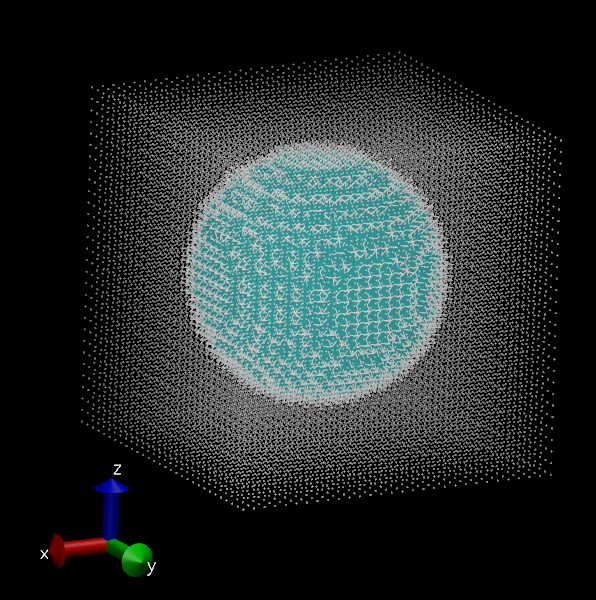
\includegraphics[scale=0.29]{sphere.png}}
  \subfigure[Cylinder]{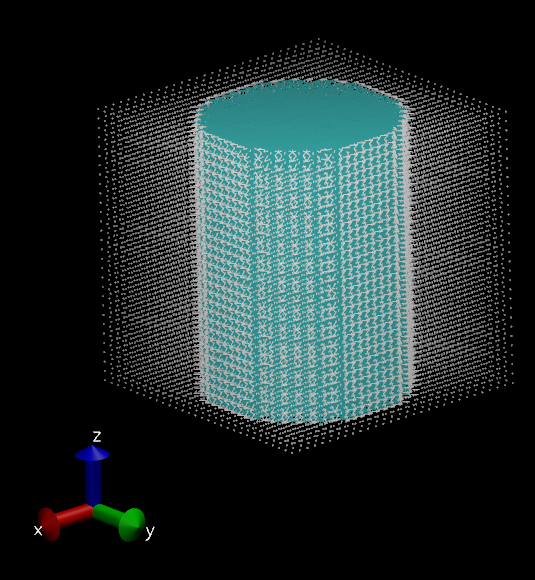
\includegraphics[scale=0.3]{cylinder.png}}
  \subfigure[Cube]{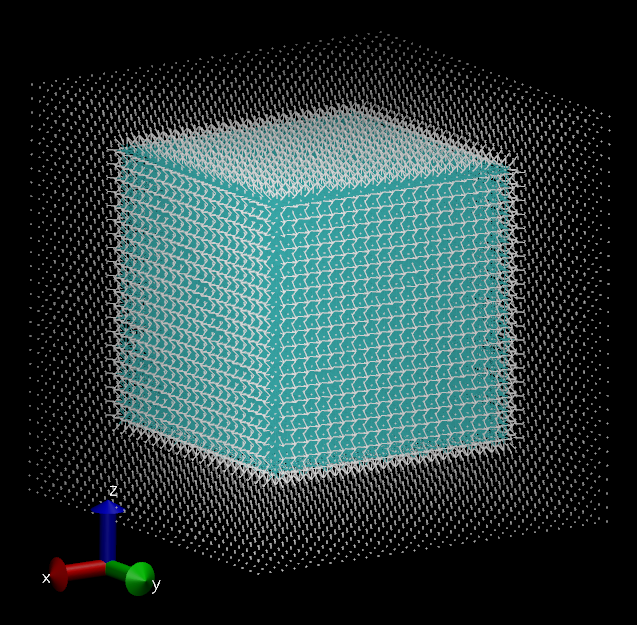
\includegraphics[scale=0.28]{cube.png}}
  \caption{Definition of the "active" (blue) and "unactive" (white) domains. 3D Box $30\times 30\times 30$ bohr radius; $30 \times 30 \times 30$ nodes; radius of the computational domaine: $15$ bohr radius.}
  \label{fig:domain3D}
\end{figure}

\begin{figure}
  \centering
  {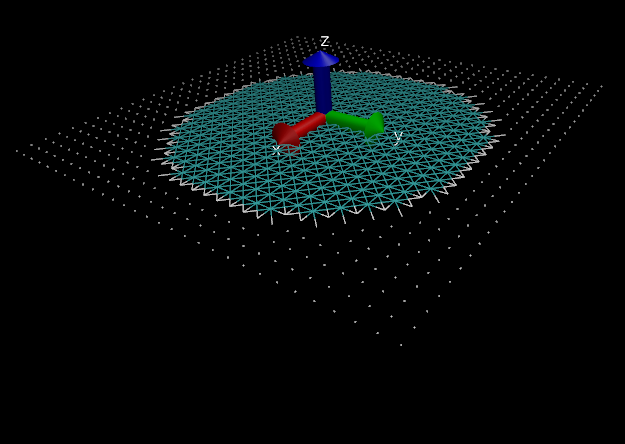
\includegraphics[scale=0.29]{circle.png}}
  \caption{Definition of the "active" (blue) and "unactive" (white) domains. 2D Box $30\times 30$ bohr radius; $30 \times 30$ nodes; radius of the computational domaine: $15$ bohr radius.}
  \label{fig:domain2D}
\end{figure}
The mesh is defined by calling the subroutine \verb+new_mesh(mesh,param)+ (in \verb+mesh.f90+).
The mesh, containing $N=N_x\times N_y\times N_z$ nodes, consists in two kind of nodes: the ``active'' nodes, belonging to the computational domain, and the ``unactive'' ones, belonging to the boundaries domain (figs.\,\ref{fig:domain3D} and \ref{fig:domain2D}). The ``active'' nodes are the nodes where we will compute quantities such as wavefunctions, potentials, ... while the ``unactive'' nodes are the nodes where all these quantities are constant.
Example of ``unactive'' nodes is the nodes located in the outer edge of the box defining the shape of the space we consider. At these locations, the value of the wavefunction is zero in the case of isolated systems.
The type of any node of the space is determined by the subroutine \verb+set_nodes(mesh)+:
\begin{itemize}
\item if the node $(i,j,k$) belongs to the computational domain, an single positive index $n$ is assigned to the node; each index $n$ corresponds to an single set $(i,j,k)$ of the space.
  \begin{eqnarray}
  (x,y,z)    &\rightarrow (i,j,k)    \rightarrow & n, \\
  \phi(x,y,z)&\rightarrow \phi_{i,j,k}\rightarrow & \phi_n, 
\end{eqnarray}
The total number of nodes inside the computational domain is $n_{active}$.

  \item if the node $(i,j,k)$ belongs to the boundaries domain, its index $n$ is set to $-1$.
\end{itemize}
The computational and boundaries domains are defined thanks to parameters decribing the shape  and the size of the computational box (\verb+mesh%box%shape+, \verb+mesh%box%center+, \verb+mesh%box%radius+)


From equations\,(\ref{eq:2}) and by using the application $  (x,y,z)\rightarrow (i,j,k)    \rightarrow  n$, solving the Schr\"odinger equation\,(\ref{eq:1}) is equivalent to solve an eigenvalues problem $H|\phi>=\epsilon|\phi>$; the vector $|\phi>$ is an eigenvector to be determined, corresponding to the eigenvalue $\epsilon$.

For each node $(i,j,k)$, the list of neighbors ($(i\pm1,j,k)$, $(i,j\pm 1,k)$, $(i,j,k\pm 1)$ in the case given here)  involved in equations\,(\ref{eq:2}) is given by the matrix \verb+mesh%node(nactive)%list_neighbors(:)+ \\ (\verb+mesh%node(nactive)%n_neighbors+ contains the number of neighbors for each node $(i,j,k)$).
These lists are set in the   subroutine \verb+compute_list_neighbors(mesh)+.

%A main interest of the application $  (x,y,z)\rightarrow (i,j,k)    \rightarrow  n$ is that it transforms a problem 


\section{Electrostatic potential}

There two ways to compute the electrostatic potential of the charge distribution, $\rho(\bm{r})$, of the electron in the system:
\begin{itemize}
\item by solving the Poisson equation, $\nabla\,U(\bm{r})=-4\pi\rho(\bm{r})$ (Hartree a.\,u.),
\item by solving the integral equation, $U(\bm{r})=\int\mathrm{d}\bm{r}^\prime\rho(\bm{r}^\prime)\frac{1}{|\bm{r}-\bm{r}^\prime|}$.
\end{itemize}
Solving the integral equation is the simplest way to proceed but it is also the most inefficient because it needs to integrate the equation for each point belonging to the grid.

Using the Poisson equation is a more efficient way to proceed. In the framework of the finite difference method, in three dimensions (3D), the Poisson equation has the form
\begin{equation}
  \frac{U_{i-1,j,k}-2U_{i,j,k}+U_{i+1,j,k}}{(\Delta\,x)^2}+
  \frac{U_{i,j-1,k}-2U_{i,j,k}+U_{i,j+1,k}}{(\Delta\,y)^2}+
  \frac{U_{i,j,k-1}-2U_{i,j,k}+U_{i,j,k+1}}{(\Delta\,z)^2}=-4\pi\rho_{i,j,k}.
\end{equation}
For each active node, the replacement of the second derivative of the electrostatic potential by a sum of functions leads to a linear systems of algebrais equations coupling the different value $U_{i,j,k}$,
\begin{equation}
  L|U>=-4\pi|\rho>.
\end{equation}
$L$ is the Laplace matrix.
% \begin{equation}
%   L=\left(\begin{array}{ccccccccccc}
%             \ldots & 0 & \frac{1}{(\Delta\,x)^2} &  -2\left(\frac{1}{(\Delta\,x)^2}+\frac{1}{(\Delta\,y)^2}+\frac{1}{(\Delta\,z)^2}\right) &  \frac{1}{(\Delta\,x)^2} & 0 &\ldots & \frac{1}{(\Delta\,y)^2} & \ldots & \frac{1}{(\Delta\,z)^2}& \ldots\\
%             \ldots & 0 & 0& \frac{1}{(\Delta\,x)^2} &  -2\left(\frac{1}{(\Delta\,x)^2}+\frac{1}{(\Delta\,y)^2}+\frac{1}{(\Delta\,z)^2}\right) &  \frac{1}{(\Delta\,x)^2} &\ldots & \frac{1}{(\Delta\,y)^2} & \ldots & \frac{1}{(\Delta\,z)^2}& \ldots\\
%           \end{array}
%           \right)
% \end{equation}

Note that for the active nodes located at the edge of the active domain, the replacement of the second derivative by a sum of function needs to take into account the unactive nodes located at the edge of the unactive. For example, for the node $(i,j,k)$, 
\begin{equation}
  \frac{U_{i-1,j,k}^*-2U_{i,j,k}+U_{i+2,j,k}}{(\Delta\,x)^2}+
  \frac{U_{i,j-1,k}-2U_{i,j,k}+U_{i,j+1,k}}{(\Delta\,y)^2}+
  \frac{U_{i,j,k-1}-2U_{i,j,k}+U_{i,j,k+1}}{(\Delta\,z)^2}=-4\pi\rho_{i,j,k}
\end{equation}
the node $U_{i-1,j,k}^*$ belongs to the unactive domain and imposes a boundary condition. Note that only a part of the unactive domain is involved in the boundary conditions. This part of the unactive domain is noted $\Omega$ in the following.
The unactive nodes involved in the boundary conditions are listed in the data type \verb+t_node+: for each active node, the integer \verb+mesh%node(:)%n_bound+ gives the number of neigbors unactive nodes contributing to the boundary conditions (their index is given in \verb+mesh%node(:)%list_bound(:)+).

Then
\begin{equation}
  \frac{-2U_{i,j,k}+U_{i+2,j,k}}{(\Delta\,x)^2}+
  \frac{U_{i,j-1,k}-2U_{i,j,k}+U_{i,j+1,k}}{(\Delta\,y)^2}+
  \frac{U_{i,j,k-1}-2U_{i,j,k}+U_{i,j,k+1}}{(\Delta\,z)^2}=-4\pi\rho_{i,j,k}-  \frac{U_{i-1,j,k}^*}{(\Delta\,x)^2}
\end{equation}
\begin{equation}
  -2\left(\frac{1}{(\Delta\,x)^2}+\frac{1}{(\Delta\,y)^2}+\frac{1}{(\Delta\,z)^2}\right)U_{i,j,k}+
  \frac{U_{i+2,j,k}}{(\Delta\,x)^2}+
  \frac{U_{i,j-1,k}}{(\Delta\,y)^2}+
  \frac{U_{i,j+1,k}}{(\Delta\,y)^2}+
  \frac{U_{i,j,k-1}}{(\Delta\,z)^2}+
  \frac{U_{i,j,k+1}}{(\Delta\,z)^2}
  =-4\pi\rho_{i,j,k}-  \frac{U_{i-1,j,k}^*}{(\Delta\,x)^2}
\end{equation}


\begin{equation}
  L|U>=-4\pi|\rho>-|b>.
\end{equation}

$|b>$ is the vector containing the boundary conditions, \emph{i.\,.e}, the values of the electrostatic potential at the edge of th
e active domain.

Now the question is: how to get the values of the electrostatic potential at the unactive point edge of the unactive domain in

\newpage

\section{Structure of the input file}

The input file is provided directly from the command line: \verb+./Hbinitio.x inp_davidson+ for example.

It must be ended by the line \verb+cmd=end+ to indicate the end of the file.

\newpage

\section{Structure of the code}



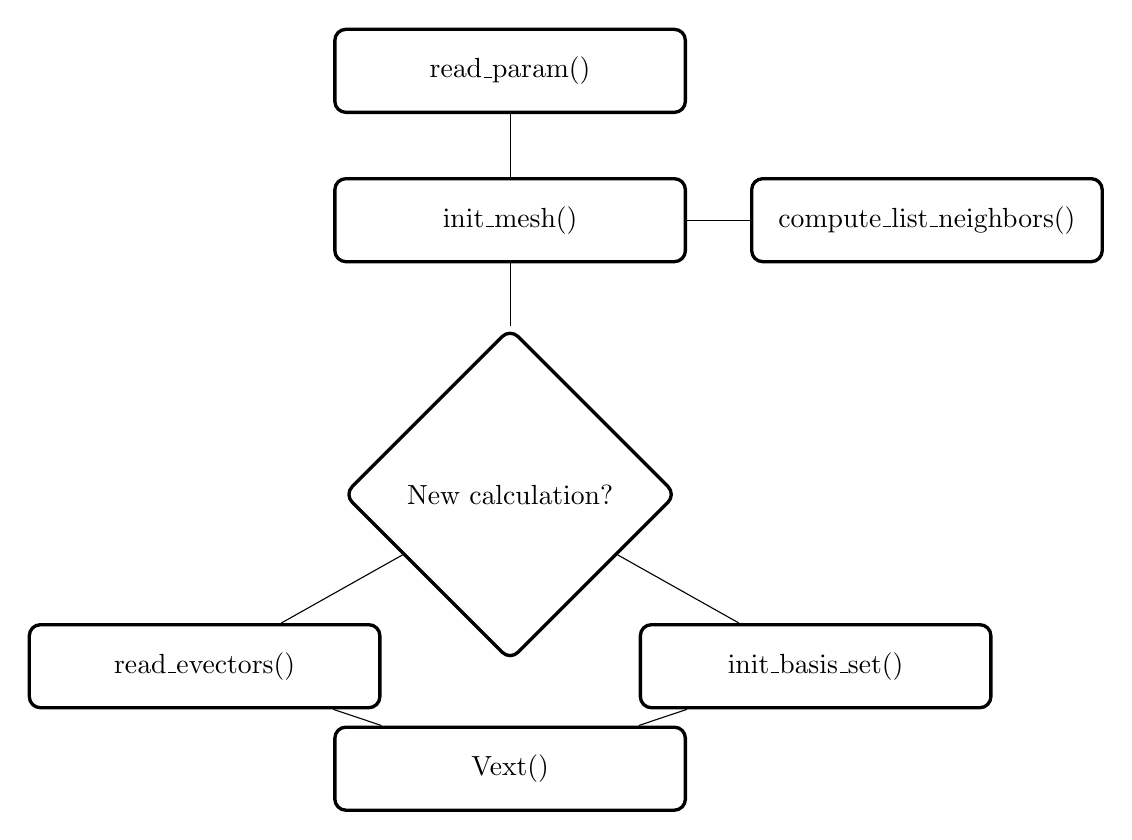
\begin{tikzpicture}[node distance=.8cm,start chain=going below,]
  \node[boite,join](read_param) {read\_param()};
  \node[boite,join](init_mesh) {init\_mesh()};
  \node[boite,](compute_list_neighbors)[right=of init_mesh] {compute\_list\_neighbors()};
  \draw[line] (init_mesh) edge (compute_list_neighbors);
  \node[boiteif](init_evec)[below=of init_mesh] {New calculation?};
  \draw[line] (init_mesh) edge (init_evec);
  \node[boite,](init_evec2)[below right= of init_evec] {init\_basis\_set()};
  \draw[line] (init_evec) edge (init_evec2);
  \node[boite,](init_evec3)[below left= of init_evec] {read\_evectors()};
  \draw[line] (init_evec) edge (init_evec3);
  \node[boite,](Vext)[below=of init_evec] {Vext()};
  \draw[line] (init_evec2) edge (Vext);
  \draw[line] (init_evec3) edge (Vext);
 \end{tikzpicture}



\section{Dealing with the perturbation}

\subsection{Real-space representation of the resolvent of the Hamiltonian, $\hat{H}$}

 
A way to compute the electron density, $n(\bm{r})$, is to resort to the identity relating the density matrix of a system, $\rho(\bm{r},\bm{r}^\prime)$, with its one-electron Green's function:
\begin{equation}
  G(\bm{r},\bm{r}^\prime;\epsilon)=<\bm{r}|\hat{G}(\epsilon)|\bm{r}^\prime>=<\bm{r}|\frac{1}{\epsilon-\hat{H}}|\bm{r}^\prime>
\end{equation}

$n(\bm{r})=\rho(\bm{r},\bm{r})$

Baroni and Giannozzi\cite{baroni1991} introduced a Green's function method which employs the finite difference and a real-space grid.

Using the Green's method needs to calculate the inverse of $(\epsilon-\hat{H})$ which may be an huge task.
Iterative algorithms, such as the Davidson's one, used to solve elliptic partial differential equations could in principle be used to calculate the inverse of   $(\epsilon-\hat{H})$  (in the Davidson's method they are used to compyte de $|delta>$ vector from the residual).
However, for the Green's method, we don't need to get the \emph{full} inverse matrix but only the diagonal element of the inverse.

Haydock, Heine and Kelly\cite{haydock1980,giannozzi1988} developped a convenient way to compute a \emph{single} diagonal element of the Green's function: the recursion method.
In the recursion method, diagonal elements of the Green's function, $<\phi_0|\hat{G}|\phi_0>$, are expressed in terms of a continuous fraction whose coefficients are calculated from a chain of orthogonal states recursively generated from $|\phi_0>$:


\section{Sources}
\label{Sources}


 
\begin{verbatim}
#! /bin/bash
####SBATCH -p public
#SBATCH -p grant -A g2018a7
###SBATCH -p grantgpu -Ag1018a7
#SBATCH -n 64 -tasks-per-node=64
#SBATCH -t 2:00:00                # Le job sera tue au bout de 1h
####SBATCH --mail-user=herve.bulou@ipcms.unistra.fr
#####SBATCH --mem=4096                # Quantite memoire demandee par noeud en Mo (unite obligatoire)


export OMP_NUM_THREADS=64
time ./Hbinitio.x

\end{verbatim}

\begin{verbatim}
module time_tracking
  implicit none
  type t_time
     real :: start,end,start_loc,end_loc
  end type t_time
contains
  ! -----------------------------------------------
  subroutine time_tracking_init(time_spent)
    implicit none
    type(t_time)::time_spent
    call cpu_time(time_spent%start)
    open(unit=1,file="dbg.dat",form='formatted',status='unknown')
    write(1,*)
    close(1)
  end subroutine time_tracking_init
  subroutine time_tracking_write(iloop,time_spent,text)
    integer :: iloop
    type(t_time)::time_spent
    character (len=*) :: text
    open(unit=1,file="dbg.dat",form='formatted',status='unknown',access='append')
    write(1,'(A50,I4,F12.6,F12.6,F12.6)') text,iloop,time_spent%end_loc,&
         time_spent%start_loc,time_spent%end_loc-time_spent%start_loc
    close(1)
  end subroutine time_tracking_write
end module time_tracking

  ! !!!!!!!!!!!!!!!!!!!!!!!!!!!!!!!!!!!!!!!!!!!!!!!!!!!!!!!!!!!!!!!!!!!!!!!!!!!!!!!!!!!!!!!!!!!!!!!!!!!!!!!
  ! !!!!!!!!!!!!!!!!!!!!!!!!!!!!!!!!!!!!!!!!!!!!!!!!!!!!!!!!!!!!!!!!!!!!!!!!!!!!!!!!!!!!!!!!!!!!!!!!!!!!!!!
  ! !!!!!!!!!!!!!!!!!!!!!!!!!!!!!!!!!!!!!!!!!!!!!!!!!!!!!!!!!!!!!!!!!!!!!!!!!!!!!!!!!!!!!!!!!!!!!!!!!!!!!!!
  ! !!!!!!!!!!!!!!!!!!!!!!!!!!!!!!!!!!!!!!!!!!!!!!!!!!!!!!!!!!!!!!!!!!!!!!!!!!!!!!!!!!!!!!!!!!!!!!!!!!!!!!!
  ! !!!!!!!!!!!!!!!!!!!!!!!!!!!!!!!!!!!!!!!!!!!!!!!!!!!!!!!!!!!!!!!!!!!!!!!!!!!!!!!!!!!!!!!!!!!!!!!!!!!!!!!
  ! !!!!!!!!!!!!!!!!!!!!!!!!!!!!!!!!!!!!!!!!!!!!!!!!!!!!!!!!!!!!!!!!!!!!!!!!!!!!!!!!!!!!!!!!!!!!!!!!!!!!!!!
program Hbinitio
  !$ use OMP_LIB
  use time_tracking
  implicit none
!  include 'mpif.h'
  type t_GramSchmidt
     integer :: nindep
     integer :: ndep ! number of linear dependencies discovered
  end type t_GramSchmidt
  type t_mesh
     integer :: Nx,Ny,Nz,N
     integer,allocatable :: list_neighbors(:,:),n_neighbors(:)
     double precision :: dx,dy,dz,dv
     double precision :: center(3)
  end type t_mesh
  type(t_mesh) :: mesh
  type t_cvg
     integer,allocatable:: list_cvg(:)
     integer :: ncvg
     double precision :: ETA
     integer :: nvec_to_cvg 
  end type t_cvg
  type(t_cvg) :: cvg
  type(t_time) :: time_spent
  type t_param
     logical::restart
     integer::ieof
     integer::loopmax
     integer::nvecini
     integer::nvecmax
     integer::Nx
     integer::nvec_to_cvg
     double precision :: ETA
     double precision::box_width
  end type t_param
  type(t_param)::param
  integer :: nvec
  integer,parameter :: seed = 86456
  double precision,allocatable :: V(:,:) ! wavefunctions
  double precision,allocatable :: Sprev(:),dS(:) ! eigenvalues
  double precision,allocatable :: pot_ext(:) ! external potential
  integer :: iloop
  character (len=1024) :: filecube
  character (len=1024)::line
  integer :: i

!  integer::ierr,my_id,num_procs
  ! !!!!!!!!!!!!!!!!!!!!!!!!!!!!!!!!!!!!!!!!!!!!!!

  call time_tracking_init(time_spent)

!  call mpi_init(ierr )
!  call MPI_COMM_RANK (MPI_COMM_WORLD, my_id, ierr)
!  call MPI_COMM_SIZE (MPI_COMM_WORLD, num_procs, ierr)

  call read_param(param)
  call init_mesh(mesh,param)  

!  nvecini=2
  nvec=param%nvecini
  allocate(V(mesh%N,nvec))
!  param%restart=.TRUE.
!  param%restart=.FALSE.
  if (.not.(param%restart))   then
     print *,"new calculation"
     call init_basis_set(V,nvec,seed,mesh)
  else
     print *,'restart an old calculation'
     call read_evectors(V,mesh,nvec)
  end if
  allocate(pot_ext(mesh%N))
  call Vext(mesh,pot_ext)
  
  open(unit=1,file="eigenvalues.dat",form='formatted',status='unknown'); write(1,*);  close(1)
  
  iloop=1
  cvg%ncvg=0
  cvg%nvec_to_cvg=param%nvec_to_cvg
  cvg%ETA=param%ETA
  allocate(Sprev(param%nvecini))
  allocate(dS(param%nvecini))
  Sprev(:)=0.0
  dS(:)=0.0
  do while((iloop.le.param%loopmax).and.(cvg%ncvg.lt.cvg%nvec_to_cvg))
     write(*,'(A)') 'Main > #######################################'     
     write(*,'(A,I4,A)') 'Main > ############ scf loop=',iloop,' ############'
     write(*,'(A)') 'Main > #######################################'     
     call davidson(nvec,V,mesh,param%nvecini,iloop,cvg,pot_ext,time_spent)
  end do
  call save_evectors(V,mesh,param%nvecini)
  do i=1,param%nvecini
     write(filecube,'(a,i0,a)') 'evec',i,'.cube'
     call norm(mesh,V(:,i))
     call save_cube(V(:,i),filecube,mesh)
  end do
  deallocate(V)
  deallocate(Sprev)
  deallocate(dS)
  deallocate(pot_ext)
  call free_mesh(mesh)
  call cpu_time(time_spent%end)
  if (cvg%ncvg.ge.cvg%nvec_to_cvg) print *,'Main > Job DONE !'
  print '("Main > Total Time = ",e16.6," seconds.")',time_spent%end-time_spent%start
!  call mpi_finalize(ierr)
  ! !!!!!!!!!!!!!!!!!!!!!!!!!!!!!!!!!!!!!!!!!!!!!!!!!!!!!!!!!!!!!!!!!!!!!!!!!!!!!!!!!!!!!!!!!!!!!!!!!!!!!!!
  ! !!!!!!!!!!!!!!!!!!!!!!!!!!!!!!!!!!!!!!!!!!!!!!!!!!!!!!!!!!!!!!!!!!!!!!!!!!!!!!!!!!!!!!!!!!!!!!!!!!!!!!!
  ! !!!!!!!!!!!!!!!!!!!!!!!!!!!!!!!!!!!!!!!!!!!!!!!!!!!!!!!!!!!!!!!!!!!!!!!!!!!!!!!!!!!!!!!!!!!!!!!!!!!!!!!
  ! !!!!!!!!!!!!!!!!!!!!!!!!!!!!!!!!!!!!!!!!!!!!!!!!!!!!!!!!!!!!!!!!!!!!!!!!!!!!!!!!!!!!!!!!!!!!!!!!!!!!!!!
  ! !!!!!!!!!!!!!!!!!!!!!!!!!!!!!!!!!!!!!!!!!!!!!!!!!!!!!!!!!!!!!!!!!!!!!!!!!!!!!!!!!!!!!!!!!!!!!!!!!!!!!!!
  ! !!!!!!!!!!!!!!!!!!!!!!!!!!!!!!!!!!!!!!!!!!!!!!!!!!!!!!!!!!!!!!!!!!!!!!!!!!!!!!!!!!!!!!!!!!!!!!!!!!!!!!!
contains
  ! --------------------------------------------------------------------------------------
  !
  !              read_param()
  !
  ! --------------------------------------------------------------------------------------
  subroutine read_param(param)
    implicit none
    type(t_param)::param
    integer::lline,eqidx
    double precision, parameter :: pi=3.1415927

    param%ieof=0
    param%loopmax=1000
    param%restart=.FALSE.
    param%nvecini=20
    param%nvecmax=41
    param%Nx=30
    param%nvec_to_cvg=20
    param%ETA=1.0e-3
    param%box_width=pi/sqrt(2.0)
    open(unit=1,file='inp',form='formatted')
    do while(.not.(is_iostat_end(param%ieof)))
       read(1,*,iostat=param%ieof) line
       lline=len_trim(line)
       eqidx=index(line,"=")
       print *,'###',eqidx,lline
       if(line(1:eqidx-1).eq."restart") then
          if(line(eqidx+1:lline).eq.'.TRUE.') then
             param%restart=.TRUE.
          else
             param%restart=.FALSE.
          end if
       end if
       if(line(1:eqidx-1).eq."loopmax") then
          read(line(eqidx+1:lline),*) param%loopmax
       end if
       if(line(1:eqidx-1).eq."nvecini") then
          read(line(eqidx+1:lline),*) param%nvecini
       end if
       if(line(1:eqidx-1).eq."nvecmax") then
          read(line(eqidx+1:lline),*) param%nvecmax
       end if
       if(line(1:eqidx-1).eq."Nx") then
          read(line(eqidx+1:lline),*) param%nx
       end if
       if(line(1:eqidx-1).eq."ETA") then
          read(line(eqidx+1:lline),*) param%ETA
       end if
       if(line(1:eqidx-1).eq."nvec_to_cvg") then
          read(line(eqidx+1:lline),*) param%nvec_to_cvg
       end if
       if(line(1:eqidx-1).eq."box_width") then
          read(line(eqidx+1:lline),*) param%box_width
       end if
       line=''
    end do
    close(1)


    print *,'#restart=',param%restart
    print *,'#loopmax=',param%loopmax
    print *,'#nvecini=',param%nvecini
    print *,'#nvecmax=',param%nvecmax
    print *,'#ETA=',param%ETA
    print *,'#nvec_to_cvg=',param%nvec_to_cvg
    print *,'#box_width=',param%box_width
    print *,'#Nx=',param%nx
    print *,'#dh=',param%box_width/(param%Nx+1)

  end subroutine read_param
  ! --------------------------------------------------------------------------------------
  !
  !              save_evectors()
  !
  ! --------------------------------------------------------------------------------------
  subroutine save_evectors(V,m,nvecini)
    implicit none
    type(t_mesh)::m
    double precision :: V(:,:)
    integer::nvecini,i,j
    open(unit=1,file="evectors.dat",form='formatted',status='unknown')
    do i=1,m%N
       write(1,*) (V(i,j),j=1,nvecini)
    end do
    close(1)
  end subroutine save_evectors
  ! --------------------------------------------------------------------------------------
  !
  !              read_evectors()
  !
  ! --------------------------------------------------------------------------------------
  subroutine read_evectors(V,m,nvecini)
    implicit none
    type(t_mesh)::m
    double precision :: V(:,:)
    integer::nvecini,i,j
    open(unit=1,file="evectors.dat",form='formatted',status='unknown')
    do i=1,m%N
       read(1,*) (V(i,j),j=1,nvecini)
    end do
    close(1)
  end subroutine read_evectors
  ! --------------------------------------------------------------------------------------
  !
  !              norm()
  !
  ! --------------------------------------------------------------------------------------
  subroutine  norm(m,evec) 
    implicit none
    double precision :: evec(:),normloc
    double precision, external :: ddot
    type(t_mesh)::m
    normloc=sqrt(m%dv*ddot(m%N,evec(:),1,evec(:),1))
    call dscal(m%N,normloc,evec(:),1)
  end subroutine norm
  ! --------------------------------------------------------------------------------------
  !
  !              Vext()
  !
  ! --------------------------------------------------------------------------------------
  subroutine Vext(m,pot_ext)
    implicit none
    type(t_mesh) :: m
    double precision :: pot_ext(:)
    double precision :: pts(3),rsqr
    
    character (len=1024) :: filename
    integer :: i,j,k,nn
    do k=1,m%Nz
       pts(3)=k*m%dz
       do i=1,m%Nx
          pts(1)=i*m%dx
          do j=1,m%Ny
             pts(2)=j*m%dy
             rsqr=(pts(1)-m%center(1))**2+(pts(2)-m%center(2))**2+(pts(3)-m%center(3))**2
             nn=j+(i-1)*m%Ny+(k-1)*m%Ny*m%Nx
             pot_ext(nn)=10*rsqr
          end do
       end do
    end do
    filename='pot_ext.cube'
    call save_cube(pot_ext,filename,m)
    !stop
  end subroutine Vext
  ! --------------------------------------------------------------------------------------
  !
  !              DAVIDSON()
  !
  ! --------------------------------------------------------------------------------------
  subroutine davidson(nvec,V,m,nvecini,iloop,cvg,pot_ext,time_spent)
    implicit none
    integer :: nvec,nvecini,iloop
    double precision,allocatable :: V(:,:),pot_ext(:)
    type(t_mesh) :: m
    type(t_cvg)::cvg
    type(t_time)::time_spent
    
    double precision,allocatable :: S(:) ! eigenvalues
    double precision,allocatable :: T(:,:) ! reduced matrix T
    double precision,allocatable :: VRitz(:,:) ! Ritz's vectors
    double precision,allocatable :: residual(:,:) ! residual
    double precision,allocatable :: delta(:,:) ! delta vectors
    double precision,allocatable :: Vnew(:,:) ! Vnew
    integer :: i
    integer :: ndelta
    integer :: newnvec
    type(t_GramSchmidt)::GS
    ! T (reduced matrix) computing
    allocate(T(nvec,nvec))
    call cpu_time(time_spent%start_loc)
    call compute_T(T,V,nvec,m,pot_ext)
    call cpu_time(time_spent%end_loc)
    call time_tracking_write(iloop,time_spent,'Davidson -> compute_T')
    
    ! Diagonatilzation of T
    allocate(S(nvec))

    call cpu_time(time_spent%start_loc)
    call diagonalization(S,T,nvec)
    call cpu_time(time_spent%end_loc)
    call time_tracking_write(iloop,time_spent,'Davidson -> Diagonalization')

    
    dS(:)=S(1:nvecini)-Sprev(:)
    Sprev(:)=S(1:nvecini)
    do i=1,nvecini
       write(*,'(A,I6,A,F12.6,A,E12.2,A)') 'Main > Eigenvalue(',i,'): ',S(i),'(',dS(i),')'
    end do
    !call cpu_time(inter)
    open(unit=1,file="eigenvalues.dat",form='formatted',status='unknown',access='append')
    write(1,*) iloop,S(1:nvecini)
    close(1)
    ! computation of the Ritz's vectors
    allocate(VRitz(m%N,nvec))

    call cpu_time(time_spent%start_loc)
    call Ritz(VRitz,V,T,nvec)
    call cpu_time(time_spent%end_loc)
    call time_tracking_write(iloop,time_spent,'Davidson -> Diagonalization')

    
    ! computation of residual
    allocate(residual(m%N,nvec))
    allocate(cvg%list_cvg(nvec))
    cvg%list_cvg(:)=0
    cvg%ncvg=0
    

    call cpu_time(time_spent%start_loc)
    call compute_residual(residual,VRitz,S,nvec,cvg,m,pot_ext)
    call cpu_time(time_spent%end_loc)
    call time_tracking_write(iloop,time_spent,'Davidson -> Residual')

    ! computation of delta
    allocate(delta(m%N,nvec))
    delta(:,:)=0.0
    !call cpu_time(inter)

    call cpu_time(time_spent%start_loc)
    call compute_delta(delta,residual,S,nvec,cvg,m,ndelta,pot_ext)
    call cpu_time(time_spent%end_loc)
    call time_tracking_write(iloop,time_spent,'Davidson -> Delta')

    
    deallocate(V)
    allocate(V(m%N,nvec+ndelta))
    V(:,1:nvec)=VRitz(:,:)
    print *,'ndelta=',ndelta
    print *,'nvec=',nvec
    V(:,nvec+1:nvec+ndelta)=delta(:,:ndelta)
    allocate(Vnew(m%N,nvec+ndelta))
    newnvec=nvec+ndelta
    GS%nindep=nvec
    !call cpu_time(inter)
    call GramSchmidt(Vnew,V,newnvec,m,GS)    
    ! call cpu_time(inter2);     call dbg(iloop,inter,inter2,'GS')
    
    print *,'Main > ',GS%ndep,newnvec
    
    deallocate(V)
    if(newnvec.le.param%nvecmax) then
       nvec=newnvec
    else
       print *,'Main > restart from nvecini'
       nvec=nvecini
    end if
    allocate(V(m%N,nvec))
    V(:,:)=Vnew(:,1:nvec)
    
    !call check_ortho(V,nvec,m)
    print *,'Main > New size of the basis ',nvec
    iloop=iloop+1
    deallocate(S)
    deallocate(T)
    deallocate(VRitz)
    deallocate(residual)
    deallocate(delta)
    deallocate(Vnew)
    deallocate(cvg%list_cvg)
  end subroutine davidson
  ! --------------------------------------------------------------------------------------
  !
  !              SAVE_CUBE()
  !
  ! --------------------------------------------------------------------------------------
  subroutine save_cube(data,filename,m)
    implicit none
    double precision :: data(:)
!    integer :: idxmin,idxmax
    type(t_mesh) :: m
    character (len=1024) :: filename
    
    character(len=*),parameter :: FMT1='(I5,3F12.6)'
    integer :: i,j,k,nn,ifield
    
    open(unit=1,file=filename,form='formatted',status='unknown')
    write(1,*) ' Cubefile created from Hbinitio.f90 calculation'
    write(1,*) ' H. Bulou, November 2018'
    write(1,FMT1) 1,0.0,0.0,0.0
    write(1,FMT1) m%Nx,m%dx,0.0,0.0
    write(1,FMT1) m%Ny,0.0,m%dy,0.0
    write(1,FMT1) m%Nz,0.0,0.0,m%dz
    write(1,'(I5,4F12.6)') 1,1.0,0.0,0.0,0.0
    do k=1,m%Nz
       ifield=0
       do i=1,m%Nx
          do j=1,m%Ny
             nn=j+(i-1)*m%Ny+(k-1)*m%Ny*m%Nx               
             write(1,'(E13.5)',advance='no') data(nn)
             ifield=ifield+1
             if (mod(ifield,6).eq.0) then
                ifield=0
                write(1,*)
             end if
          end do
       end do
       write(1,*)
    end do
    close(1)
  end subroutine save_cube

  ! --------------------------------------------------------------------------------------
  !
  !              COMPUTE_DELTA()
  !
  ! --------------------------------------------------------------------------------------
  subroutine compute_delta(delta,r,lambda,nvec,cvg,m,ndelta,pot_ext)
    ! INPUT: the residual |r>, the Ritz's vectors |VRitz>, the eigenvalues lambda
    ! OUTPUT : the correction |delta> to improve the  Ritz's vectors so that to
    !          minimize the residual
    implicit none
    type(t_mesh)::m
    double precision :: lambda(:),r(:,:),delta(:,:),pot_ext(:)
    integer :: nvec,ndelta
    type(t_cvg)::cvg
    
    double precision, external :: ddot
    double precision, parameter::alpha=1.0,beta=0.0
    double precision, allocatable :: normloc
!    double precision, allocatable :: Dinv(:,:)
    integer :: i,j
    double precision :: deltasqr

    deltasqr=m%dx**2
    print *,'Delta > ---------------------'
    print *,'Delta > --- compute_delta ---'
    print *,'Delta > ---------------------'
    !delta(:,:)=0.0
   ! allocate(Dinv(m%N,m%N))
  !  Dinv(:,:)=0.0
    ndelta=0
    do i=1,nvec
       if(cvg%list_cvg(i).eq.0) then
          ndelta=ndelta+1
          do j=1,m%N
             delta(j,ndelta)=r(j,ndelta)/((3.0/deltasqr+pot_ext(j))-lambda(i))
!             Dinv(j,j)=1.0/((3.0/deltasqr+pot_ext(j))-lambda(i))
          end do
          ! see Victor Eijkhout in "Introduction to scientific and technical computing" edited by Willmore et al
          ! Chap 15 Libraries for Linear Algebra
          ! to get a comprehensive way to use dgemv
 !         call dgemv('N',m%N,m%N,alpha,Dinv,m%N,r(:,ndelta),1,beta,delta(:,ndelta),1)
          !norm=sqrt(ddot(m%N,delta(:,i),1,delta(:,i),1))
          !write(*, '(A10,I4,A2,E12.6)',advance='no') ' Delta > delta(',i,')=',norm
          !delta(:,ndelta)=delta(:,ndelta)+VRitz(:,ndelta)
          normloc=1.0/sqrt(ddot(m%N,delta(:,ndelta),1,delta(:,ndelta),1))
          call dscal(m%N,normloc,delta(:,ndelta),1)
       end if
    end do
    !deallocate(Dinv)
    print *,'Delta > ',ndelta,' new vector(s)'
  end subroutine compute_delta
    
  
  ! --------------------------------------------------------------------------------------
  !
  !              COMPUTE_RESIDUAL()
  !
  ! --------------------------------------------------------------------------------------
  subroutine compute_residual(r,VRitz,S,nvec,cvg,m,pot_ext)
    implicit none
    type(t_mesh)::m
    integer :: nvec
    double precision :: r(:,:),VRitz(:,:),S(:),pot_ext(:)
    type(t_cvg) :: cvg

    integer :: i,j,k
    double precision :: normloc
    double precision, external :: ddot        
    double precision :: deltasqr

    print *,'Residual > ------------------------'
    print *,'Residual > --- compute residual ---'
    print *,'Residual > ------------------------'
    deltasqr=m%dx**2
    r(:,:)=0.0
    cvg%ncvg=0
    do j=1,nvec
       do i=1,m%N
          r(i,j)=(3.0/deltasqr+pot_ext(i))*VRitz(i,j)
          do k=1,m%n_neighbors(i)
             r(i,j)=r(i,j)-0.5*VRitz(m%list_neighbors(i,k),j)/deltasqr
          end do
          r(i,j)=r(i,j)-S(j)*VRitz(i,j)
       end do
       normloc=ddot(m%N,r(:,j),1,r(:,j),1)
       write(*,'(A,I4,A,E12.4,A,E12.4)',advance='no') 'Residual > r(',j,')= ',normloc,'/',cvg%ETA
       if (normloc.lt.cvg%ETA) then
          cvg%ncvg=cvg%ncvg+1
          cvg%list_cvg(j)=1
          write(*,*) '--> converged'
       else
          write(*,*)
       end if
       
    end do
  end subroutine compute_residual
  
  ! --------------------------------------------------------------------------------------
  !
  !              RITZ()
  !
  ! --------------------------------------------------------------------------------------
  subroutine Ritz(Vout,Vin,y,nvec)
    implicit none
    double precision :: Vin(:,:),Vout(:,:),y(:,:)
    integer :: nvec

    integer :: i,j
    print *,'Ritz > --------------'
    print *,'Ritz > --- Ritz() ---'
    print *,'Ritz > --------------'
    do i=1,nvec
       Vout(:,i)=y(1,i)*Vin(:,1)
       do j=2,nvec
          Vout(:,i)=Vout(:,i)+y(j,i)*Vin(:,j)
       end do
    end do
  end subroutine Ritz
  
  
  ! --------------------------------------------------------------------------------------
  !
  !              DIAGONALIZATION()
  !
  ! --------------------------------------------------------------------------------------
  subroutine diagonalization(S,H,N)
    implicit none
    integer :: N
    double precision :: H(:,:),S(:)

    integer :: lwork,info
    integer :: lwmax
    double precision,allocatable::work(:)
    parameter(lwmax=100000)
    allocate(work(lwmax))
    lwork=-1
    call  dsyev('vectors','Upper',N,H,N,S,work,lwork,info)
    lwork=min(lwmax,int(work(1)))
    if (lwork.ge.lwmax) then
       write(*,*) 'Diagonalization > WARNING info = ',info
       write(*,*) 'Diagonalization > WARNING lwork=',lwork
       write(*,*) 'Diagonalization > WARNING size of work(1)',int(work(1))
       stop
    end if
    call  dsyev('vectors','Upper',N,H,N,S,work,lwork,info)
    if(info.gt.0) then
       write(*,*) "Diagonalization > WARNING The algorithm computing failed"
       stop
    end if
    deallocate(work)
  end subroutine diagonalization
  
  
  ! --------------------------------------------------------------------------------------
  !
  !              COMPUTE_T()
  !
  ! --------------------------------------------------------------------------------------
  subroutine compute_T(T,V,nvec,m,pot_ext)
    implicit none
    double precision,allocatable :: V(:,:),T(:,:),pot_ext(:)
    integer :: nvec
    type(t_mesh)::m
    
    integer :: i,j,k,l
    double precision :: deltasqr,acc
    double precision, parameter::alpha=0.0
!    double precision::beta
    
    deltasqr=m%dx**2
    !$OMP PARALLEL private(acc) 
    !$OMP DO 
    do j=1,nvec
       do i=1,nvec ! Tij
          T(i,j)=0.0
          do k=1,m%N
             acc=(3.0/deltasqr+pot_ext(k))*V(k,j) ! the potential will be added here
             do l=1,m%n_neighbors(k)
                acc=acc-0.5*V(m%list_neighbors(k,l),j)/deltasqr
!                print *, omp_get_thread_num(),i,j,k,l
             end do
             T(i,j)=T(i,j)+V(k,i)*acc
!             print *,' -> ',omp_get_thread_num(),i,j,T(i,j)
          end do
!          print *,omp_get_thread_num(),i,j,T(i,j)
       end do
    end do
    !$OMP END DO
    !$OMP END PARALLEL
!    stop
  end subroutine compute_T
  
  
  ! --------------------------------------------------------------------------------------
  !
  !              INIT_BASIS_SET()
  !
  ! --------------------------------------------------------------------------------------
  subroutine init_basis_set(V,nvec,seed,m)
    implicit none
    integer :: nvec,seed
    double precision,allocatable :: V(:,:)
    type(t_mesh)::m

    double precision, external :: ddot
    double precision ::normloc
    integer :: i,j
    double precision,allocatable :: Vdump(:,:)
    type(t_GramSchmidt) :: GS
    
    allocate(Vdump(m%N,nvec))
    call srand(seed)
    do i=1,nvec
       do j=1,m%N
          Vdump(j,i)=rand()
       end do
    end do
    do i=1,nvec
       normloc=ddot(m%N,Vdump(:,i),1,Vdump(:,i),1)
       normloc=1.0/sqrt(normloc)
       call dscal(m%N,normloc,Vdump(:,i),1)
    end do
    GS%nindep=1
    call GramSchmidt(V,Vdump,nvec,m,GS)

    deallocate(Vdump)
  end subroutine init_basis_set
  ! -----------------------------------------------
  ! Ref.: D. G. Clayton "Gram-Schmidt Orthogonalization", J. Roy. Stat. Soc. C 20, 335 (1971)
  subroutine GramSchmidt(Vout,Vin,nvec,m,GS)
    implicit none
    integer ::  nvec
    double precision,allocatable :: Vin(:,:),Vout(:,:)
    type(t_mesh)::m
    type(t_GramSchmidt) :: GS
    
    integer :: i,k,i0
    double precision, parameter :: ETA=1.0e-6
    double precision,allocatable :: a(:)
    double precision :: normloc
    double precision, external :: ddot

    allocate(a(nvec))
    print *,'GS> ----------------------'
    print *,"GS> Gram-Schmidt algorithm"
    print *,'GS> ----------------------'
    print *,'GS> ',nvec,' vectors to orthogonalize'
    print *,'GS> ',GS%nindep,' vectors are already orthogonalized'
    Vout(:,1:GS%nindep)=Vin(:,1:GS%nindep)
    GS%ndep=0 
    i0=GS%nindep
    do i=i0+1,nvec
       Vout(:,GS%nindep+1)=Vin(:,i)
       do k=1,GS%nindep
          ! We compute the projection of Vini(:,i) on V(:,1-nindep)
          a(k)=ddot(m%N,Vout(:,k),1,Vin(:,i),1)
          !print *,'GS > ',i,k,a(k)
          ! then we remove V(:,k) from V(:,nindep+1)
          call daxpy(m%N,-a(k),Vout(:,k),1,Vout(:,GS%nindep+1),1)
       end do
       ! now wre compute the norm of V(:,nindep+1)
       normloc=sqrt(ddot(m%N,Vout(:,GS%nindep+1),1,Vout(:,GS%nindep+1),1))
       !print *,'GS > norm(',i,')=',norm
       if (normloc.le.ETA) then
          GS%ndep=GS%ndep+1 ! V(:,nindep+1) is not linearly inependent
       else
          normloc=1.0/normloc
          call dscal(m%N,normloc,Vout(:,GS%nindep+1),1)
          !              do k=2,icur
          !                 print *,'<U',k-1,'|U',i,'>=',ddot(N,V(:,k-1),1,V(:,icur),1)
          !              end do
          GS%nindep=GS%nindep+1
       end if
    end do
    print *,'GS> ',GS%ndep,' vectors linearly dependant'
    print *,'GS> ',GS%nindep,' vectors linearly independant'
    print *,'GS> Size of the basis from ',nvec,' to ',GS%nindep
    !call check_ortho(Vout,nvec,m)
    !stop
    nvec=GS%nindep
    deallocate(a)
  end subroutine GramSchmidt
  ! -----------------------------------------------
  subroutine check_ortho(P,nvec,m)
    implicit none
    integer :: nvec
    double precision :: P(:,:)
    type(t_mesh)::m

    double precision, parameter :: ETA=1.0e-6
    integer :: i,j,nfail
    double precision :: pscal
    double precision, external :: ddot
    nfail=-nvec
    print *,"--- check_ortho() ---"      
    do i=1,nvec
       do j=1,nvec
          pscal=ddot(m%N,P(:,i),1,P(:,j),1)
          write(*,'(F10.2)',advance='no') pscal
          if (pscal.gt.ETA) nfail=nfail+1
       end do
       write(*,*)
    end do
    if (nfail.gt.0) then
       print *,nfail,' fail(s)'
       stop
    end if
  end subroutine check_ortho
  

  ! -----------------------------------------------
  subroutine init_mesh(m,param)
    implicit none
    type(t_mesh)::m
    type(t_param)::param
    double precision:: Lwidth 

    Lwidth=param%box_width
    m%Nx=param%Nx
!    m%Nx=5
    m%Ny=m%Nx
    m%Nz=m%Nx
    m%N=m%Nx*m%Ny*m%Nz

    m%dx=Lwidth/(m%Nx+1)
    m%dy=Lwidth/(m%Ny+1)
    m%dz=Lwidth/(m%Nz+1)
    m%dv=m%dx*m%dy*m%dz
    !m%dv=1.0

    m%center(1)=Lwidth/2
    m%center(2)=Lwidth/2
    m%center(3)=Lwidth/2
    
    allocate(m%n_neighbors(m%N))
    allocate(m%list_neighbors(m%N,6)) !
    m%list_neighbors(:,:)=0
    m%n_neighbors(:)=0
    call compute_list_neighbors(m)
  end subroutine init_mesh
  ! -----------------------------------------------
  subroutine free_mesh(m)
    implicit none
    type(t_mesh) :: m
    deallocate(m%n_neighbors)
    deallocate(m%list_neighbors) !
  end subroutine free_mesh
  ! -----------------------------------------------
  subroutine compute_list_neighbors(m)
    implicit none
    type(t_mesh) :: m
    integer::i,j,k,nn
    !integer,allocatable::n_neighbors(:),list_neighbors(:,:)
    
    do k=1,m%Nz
       do i=1,m%Nx
          do j=1,m%Ny
             nn=j+(i-1)*m%Ny+(k-1)*m%Ny*m%Nx
             if (k>1) then 
                m%n_neighbors(nn)=m%n_neighbors(nn)+1
                m%list_neighbors(nn,m%n_neighbors(nn))=nn-m%Nx*m%Ny
             end if
             if (k<m%Nz) then 
                m%n_neighbors(nn)=m%n_neighbors(nn)+1
                m%list_neighbors(nn,m%n_neighbors(nn))=nn+m%Nx*m%Ny
             end if
             if (i>1) then 
                m%n_neighbors(nn)=m%n_neighbors(nn)+1
                m%list_neighbors(nn,m%n_neighbors(nn))=nn-m%Ny
             end if
             if (i<m%Nx) then 
                m%n_neighbors(nn)=m%n_neighbors(nn)+1
                m%list_neighbors(nn,m%n_neighbors(nn))=nn+m%Ny
             end if
             if (j>1) then 
                m%n_neighbors(nn)=m%n_neighbors(nn)+1
                m%list_neighbors(nn,m%n_neighbors(nn))=nn-1
             end if
             if (j<m%Ny) then 
                m%n_neighbors(nn)=m%n_neighbors(nn)+1
                m%list_neighbors(nn,m%n_neighbors(nn))=nn+1
             end if
          end do
       end do
    end do

  end subroutine compute_list_neighbors
  
  
end program Hbinitio
\end{verbatim}

\begin{thebibliography}{1}
\bibitem{laaksonen1986} L. Laaksonen, P. Pyykko, and D. Sundholm, Compu. Phys. Rep. \textbf{4}, 313 (1986).
\bibitem{varga2011} ``Computational Nanoscience,'' (2011), K. Varga and J. A. Driscoll, Cambridge University Press.
\bibitem{mazumder2015} ``Numerical Methods for Partial Differential Equations: Finite Difference and Finite Volume Methods,'' (2015), S. Mazumder, Academic Press.
\bibitem{baroni1991} ``Towards Very Large-Scale Electronic-Structure Calculations'', S. Baroni and P. Giannozzi 1992 EPL \textbf{17} 547.
\bibitem{haydock1980} Haydock R., Heine V. and Kelly M. J., J . Phys. C, \textbf{5} (1972) 2845; \textbf{8} (1975) 2591; for a review, see: Ehrenreich, H., Seitz F. and Turnbull D. (Editors), Solid State Physics, Vol. 35 (Academic Press, New York, N.Y.) 1980.
\bibitem{giannozzi1988}  Giannozzi P., Grosso G., Moroni S. and Pastori Parravicini G., Appl. Num. Math., \textbf{4} (1988) 273.
\end{thebibliography}

\end{document}
